\documentclass[12pt]{article}

\usepackage{amsmath, amsfonts}
\usepackage{hyperref}
\usepackage{graphicx}
\usepackage{geometry}
\geometry{
	a4paper,
 	left=24mm,
 	right=24mm,
 	top=30mm,
 	bottom=35mm
}
\usepackage{color}
\definecolor{bluekeywords}{rgb}{0.13,0.13,1}
\definecolor{greencomments}{rgb}{0,0.5,0}
\definecolor{redstrings}{rgb}{0.9,0,0}
\definecolor{cyantypes}{RGB}{0,183,235}

\usepackage{listings}
\lstdefinelanguage{FSharp}%
{morekeywords=[1]{let, new, match, with, rec, open, module, namespace, type, of, member, % 
and, for, while, true, false, in, do, begin, end, fun, function, return, yield, try, %
mutable, if, then, else, cloud, async, static, use, abstract, interface, inherit, finally },
  morekeywords=[2]{double, float, int, string, List, BigInteger},
  otherkeywords={ let!, return!, do!, yield!, use!, var, select, where, order, by },
% otherkeywords={from}
  keywordstyle=[1]\color{bluekeywords},
  keywordstyle=[2]\color{cyantypes},
  sensitive=true,
  basicstyle=\ttfamily,
	breaklines=true,
  xleftmargin=\parindent,
  aboveskip=\bigskipamount,
	tabsize=4,
  morecomment=[l][\color{greencomments}]{///},
  morecomment=[l][\color{greencomments}]{//},
  morecomment=[s][\color{greencomments}]{{(*}{*)}},
  morestring=[b]",
  showstringspaces=false,
  literate={`}{\`}1,
  stringstyle=\color{redstrings},
}
\definecolor{codegreen}{rgb}{0,0.6,0}
\definecolor{codegray}{rgb}{0.5,0.5,0.5}
\definecolor{codepurple}{rgb}{0.58,0,0.82}
\definecolor{backcolour}{rgb}{0.95,0.95,0.92}
\lstdefinestyle{mystyle}{
    backgroundcolor=\color{backcolour},   
    commentstyle=\color{codegreen},
    keywordstyle=\color{magenta},
    numberstyle=\tiny\color{codegray},
    stringstyle=\color{codepurple},
    basicstyle=\footnotesize\ttfamily,
    breakatwhitespace=false,         
    breaklines=true,                 
    captionpos=b,                    
    keepspaces=true,                 
    numbers=left,                    
    numbersep=5pt,                  
    showspaces=false,                
    showstringspaces=false,
    showtabs=false,                  
    tabsize=4
}
\lstset{style=mystyle}
\begin{document}


\begin{center}

{\large F\# Tutorial\\} \vspace{2mm}
\textbf{\LARGE Pipe-Forward Operator}\\
\vspace{1.5mm}
{\Large\emph{\today}}

\end{center}


\section{Syntax, variables, functions}

\subsection*{Key concepts: } 

\begin{enumerate}
\item Having a good text editor helps you code much easier.
\item 
\begin{enumerate}
\item Once defined, a variable in F\# cannot change value (unless "mutable" is used)
\item If you need an updated value, create a new one.
\end{enumerate}
\item Different datatypes (e.g. integer and decimal-numbers) do not combine easily.
\item Defining and using functions in F\# is slightly different from math notation/ other languages.
\begin{enumerate}
\item F\# automatically detects the type of the variables (e.g. integer, double, etc.) for a function.
\item The variable types for a function will be enforced.
\end{enumerate}
\end{enumerate}

\subsection{Setting Up} 
\subsubsection{Comments}
You can use double-slash \texttt{//}, triple-slash \texttt{///}, or star-bracket \texttt{(* ...... *)} to make comments.

\begin{lstlisting}[language=FSharp]
// These words are ignored.
/// These words are ignored.
(* These words are ignored. *)
let x = 1
let y = x + 5
\end{lstlisting}

\subsubsection{F\# Interactive}

If you are using Visual Studio, you can run the code above by highlighting/selecting the code using your mouse, and press \texttt{ALT + ENTER}, or right-click and select \texttt{Execute in Interactive}.

\begin{center}
INSERT PICTURE HERE.
\end{center}
\vfill

\pagebreak

\subsubsection{Intellisense}
If you are using Visual Studio or Visual Studio Code, you can put your mouse on top of the variable name \texttt{x} or \texttt{y}, and see that it is an \texttt{int} or integer.

This feature will help you identify what is each variable/function, and make coding easier for you. 
\begin{center}
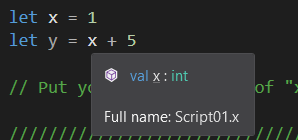
\includegraphics[width=5cm]{pictures/picture01.png}
\end{center}
\subsection{Data Type}

\subsubsection{Common data types and printing}

Some of the common types in F\# are:
\begin{center}
\begin{tabular}{|c|c|c|}
\hline Keyword & Description & Print in output:
\\ \hline \texttt{int} & Integer & \texttt{\%i}
\\ \hline \texttt{double} or \texttt{float} & Decimal numbers & \texttt{\%f}
\\ \hline \texttt{string} & Words/Sentences & \texttt{\%s}
\\ \hline \texttt{bool} & True/False & \texttt{\%b}
\\ \hline - & Other objects & \texttt{\%A} or \texttt{\%O}
\\ \hline
\end{tabular}
\end{center}

\begin{lstlisting}[language=FSharp]
let name = "John"
let age = 21
let height = 170.5

printfn "My name is: %s" name

printfn "Name: %s. Age: %i. Height: %f." name age height

printfn "His height is: %.2f" height
// %.2f for showing two decimals.
\end{lstlisting}
Output:
\begin{lstlisting}[language=FSharp]
// Output:
// My name is: John
// Name: John. Age: 21. Height: 170.500000
// His height is: 170.50
\end{lstlisting}
For example, in the second example, inside the string-format, there are \texttt{\%s, \%i, \%f}. And so, we expect a string, integer, and decimal (in that order) after the string-format specification in order to completely print the result to the output console.

\vfill

\pagebreak

\subsubsection{Equality and simple if-else}

The \texttt{let ... = ...} combination is used to assigned a value to a variable. Other than this situation, the equal sign \texttt{=} is used for equality testing. \texttt{=, <>} are used for equality/inequality testing.


\begin{lstlisting}[language=FSharp]
let valueToTest = 20
let isValueEqualToTwenty = (valueToTest = 20)

if isValueEqualToTwenty then
    printfn "Yes, the value is Twenty"
else 
    printfn "No, the value is not Twenty"
// Output: "Yes, the value is Twenty"
///////////////////////////////////////

let inputUserName = "Jack"

if inputUserName = "John" then
    printfn "Welcome back, John"
else 
    printfn "Access denied."
// Output: "Access denied."
\end{lstlisting}

In Java/C++, \texttt{==, !=} are used for comparison, and in Javascript, \texttt{===, !==} are used.

\subsubsection{Immutability}

In F\#, variables are by default immutable/unchangable. Once defined, the value of a variable cannot be changed. You can make a variable changable/mutable using the keyword \texttt{mutable} and symbol \texttt{<-}, but this is \underline{highly discouraged}. (If you use VisualStudio, then the color of the variable name will change color, warning you of potential mutable values)

\begin{center}
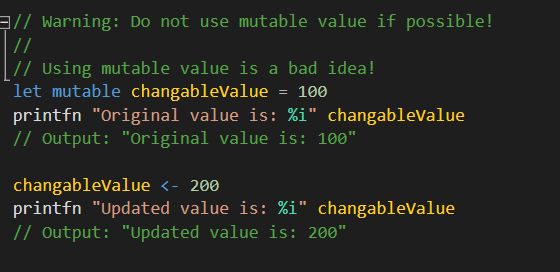
\includegraphics[width=12cm]{pictures/picture02.png}
\end{center}

\vfill

\pagebreak

If you try to update an immutable/unchangable value using \texttt{<-}, you will get an error. 

\begin{center}
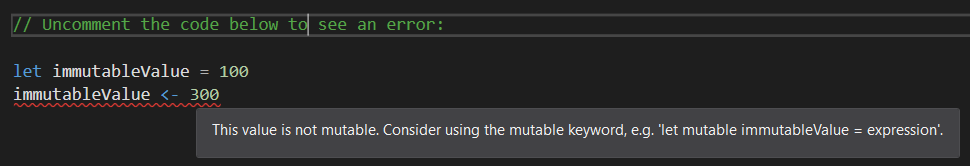
\includegraphics[width=16cm]{pictures/picture03.png}
\end{center}

\subsubsection*{Benefit of immutable/unchangable values}

Imagine the code below, with a mutable value \texttt{x}, and after thousands of lines of code later, you used \texttt{x}'s value again:

\begin{lstlisting}[language=FSharp]
let mutable x = 100
//
// Thousands of lines of code later......
// You have many lines of code in between......
// It is hard to keep track......
// Have you changed/updated x's value?
// Did you accidentally call any function that modify x?
// Can you guarantee x's value stay unchanged?
// 
//
let y = x + 1
// What is the value of y?
//
// That depends on what happens between y's definition 
// and x's definition.
\end{lstlisting}
\begin{center}
\line(1,0){400}
\end{center}

On the other hand, if \texttt{x} is immutable/unchangable:

\begin{lstlisting}[language=FSharp]
let x = 100
//
// Thousands of lines of code later......
// You have many lines of code in between......
// But because x is immutable/unchangable......
// We can be sure that x stays constant......
// And we can safely conclude that......
//
let y = x + 1
// y = 101
\end{lstlisting}
Conclusion: Use immutable/unchangable value whenever possible. AVOID mutable/changable value whenever possible.

\pagebreak

\subsubsection{(+) Operator on the same type of variable}

Integers, double, and string support the \texttt{(+)} operation:
\begin{lstlisting}[language=FSharp]

let number1 = 40
let number2 = 55
let addTwoNumbers = number1 + number2

// Remark: "float" and "double" mean the same thing in F#.
let sqrtTwoApprox = 1.414
let piApprox = 3.1415926
let addTwoDecimals = sqrtTwoApprox + piApprox

let sentenceStart = "My school is "
let schoolName = "National University of Singapore"
let combinedSentence = sentenceStart + schoolName
\end{lstlisting}
However, you cannot add an integer with a decimal in F\# directly using \texttt{(+)}, and you cannot add/concatenate a string with a number directly using \texttt{(+)}. If you use VisualStudio, then you may see an error similar to the one below.
\begin{center}
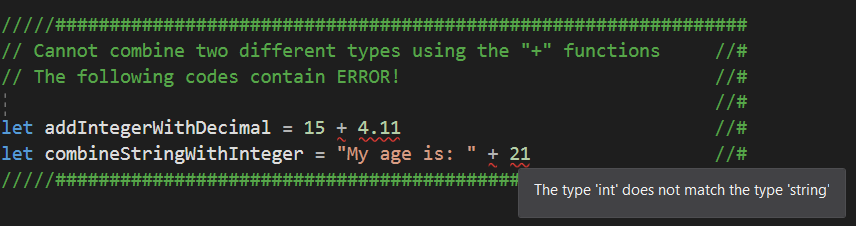
\includegraphics[width=14cm]{pictures/picture04.png}
\end{center}
Furthermore, some functions, like the square root \texttt{sqrt} and math exponent \texttt{(**)} only accepts decimal numbers:

\begin{lstlisting}[language=FSharp]
let sqrtRootOfNine = sqrt 9.0
let twoToPowerOfFive = 2.0 ** 5.0 
\end{lstlisting}
And it will cause error if you use them with integer input instead.
\begin{center}
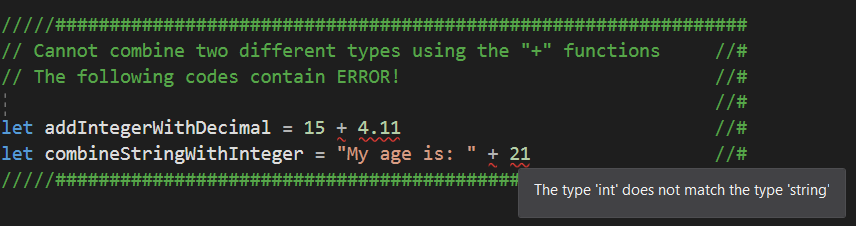
\includegraphics[width=14cm]{pictures/picture04.png}
\end{center}

\pagebreak
\subsection{Functions}

\subsubsection{One variable functions}

You can define functions using \texttt{let} followed by the inputs of your function.

\begin{lstlisting}[language=FSharp]
let f x = x + 5

let result1 = f 10
let result2 = f 20
\end{lstlisting}
Output:
\begin{lstlisting}[language=FSharp]
// val result1 : int = 15
// val result2 : int = 25
\end{lstlisting}

Notice the following:
\begin{enumerate}
\item To apply the function \texttt{f}, you do not need to use the math notation $f(x)$. You can apply the arguments by separating with a space.
\item If you hover your mouse on top of the function \texttt{f}, you will see that \texttt{f} is a function that accepts only integer \texttt{x} as the argument.
\begin{center}
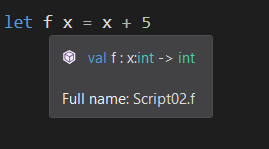
\includegraphics[width=4cm]{pictures/picture06.png}
\end{center}
\begin{enumerate}
\item This is because in the function, \texttt{x} will be added \texttt{(+)} to the integer \texttt{5}. We have seen before that we cannot use the symbol \texttt{(+)} to combine an integer with a decimal number directly. Hence, \texttt{x} has to be of type \texttt{int}.
\item As a consequence, if you try to input a decimal number to the function \texttt{f}, then it will fail:
\begin{center}
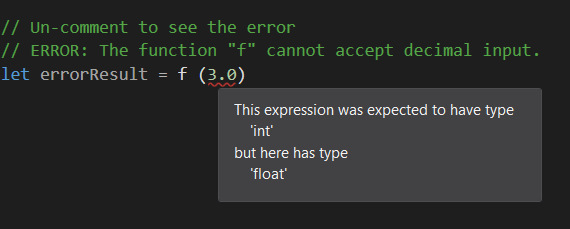
\includegraphics[width=9cm]{pictures/picture07.png}
\end{center}
\end{enumerate}
\item As mentioned, F\# automatically inferred that \texttt{x} is an integer. This is different from other languages (e.g. Java, C++) that needs you to specify the type of the variable (is it an integer? double? etc.)
 
So, you can spend less time on the tiny details (e.g. what is the variable type), and focus more on the correctness of your program.
\end{enumerate}

\pagebreak

Similarly, the following function accepts decimals/double only.

\begin{lstlisting}[language=FSharp]
let DiscountFunc originalPrice = originalPrice * 0.8

let discountedPrice = DiscountFunc 399.99
printfn "New price: %.2f" discountedPrice
// Output: "New price: 319.99"

let anotherDiscount = DiscountFunc discountedPrice
printfn "New price: %.2f" anotherDiscount
// Output: "New price: 255.99"
\end{lstlisting}
Remark: The \texttt{\%.2f} for printing 2 decimals.

This function does not accept integer values:
\begin{center}
INPUT ERROR PICTURE HERE!
\end{center}

We need to convert integer to decimal (using \texttt{double} or \texttt{float}) before using the function.

\begin{lstlisting}[language=FSharp]
let convertedPrice = double 100
let decimalResult = DiscountFunc convertedPrice
printfn "New price: %.2f" decimalResult
// Output: "New price: 80.00"
\end{lstlisting}
\begin{center}
\line(1,0){400}
\end{center}
Similarly, the following function accepts strings only.
\begin{lstlisting}[language=FSharp]
// Define a function for string.
let AddGreeting name =
    "Hello " + name

let greeting1 = AddGreeting "John"
let greeting2 = AddGreeting "Mary"
\end{lstlisting}
Output:
\begin{lstlisting}[language=FSharp]
// val greeting1 : string = "Hello John"
// val greeting2 : string = "Hello Mary"
\end{lstlisting}
And it will cause error if you try to input an integer value to this function:
\begin{center}
INPUT ERROR PICTURE HERE!
\end{center}
\pagebreak
Exercise: Write a function that calculates the area of a circle of radius $r$. 



\begin{lstlisting}[language=FSharp]
let CircleArea r =
     //
     // ... INSERT YOUR CODE HERE ...
     // Hint: Use    "System.Math.PI"
\end{lstlisting}

\subsubsection{Two variable functions}
You can define a function that takes in two variables:
\begin{lstlisting}[language=FSharp]
let g x y = 3 * x + y

let result3 = g 3 1
let result4 = g 10 2
\end{lstlisting}
\begin{lstlisting}[language=FSharp]
// val result3 : int = 10
// val result4 : int = 32
\end{lstlisting}
Notice the following:
\begin{enumerate}
\item To apply the function \texttt{g}, you do not need to use the math notation $g(x,y)$ with brackets and commas. This is different from other programming languages (e.g. Java, C++). You can apply the arguments by separating with a space.
\item If you hover your mouse on top of \texttt{g}, as seen in this picture:
\begin{center}
INPUT PICTURE HERE!
\end{center}
You will see that the variables \texttt{x, y} need to be integers.
\begin{enumerate}
\item This is because in the function, \texttt{x} will be multiplied with \texttt{3}, and then later added with \texttt{y}. As seen before, the addition and multiplication symbol \texttt{(+), (*)} only combined numbers of the same type (integers with integers, double with double)
\item As a consequence, if you input decimals into the function, it will fail:
\begin{center}
INPUT PICTURE HERE!
\end{center}
\end{enumerate}
\item Again, you can spend less time typing out the details (i.e. what are the types of \texttt{x, y}? Integer? Double?) and focus more on making your program/algorithm works, and make yourself more productive (compared to other programming languages)
\end{enumerate}

\pagebreak

Similarly, the following function accepts two decimal numbers:
\begin{lstlisting}[language=FSharp]
let CalculateNewBalance interestRate principal  = 
    principal * (1.0 + interestRate)

let balance1 = CalculateNewBalance 0.05 100000.00 
printfn "New Balance: %f" balance1
// Output: "New Balance: 105000.00"

let balance2 = CalculateNewBalance 0.03 5000.00 
printfn "New Balance: %f" balance2
// Output: "New Balance: 5150.00"
\end{lstlisting}

And it will cause error if you try to change one of the input into integer.
\begin{center}
INPUT PICTURE HERE!
\end{center}

\subsubsection{Multivariable functions}
\begin{lstlisting}[language=FSharp]
let h x y z = 3 * x + 4 * y + 5 * z

// 3*3 + 4*4 + 5*5 = 50
let result5 = h 3 4 5

// 3*1 + 4*1 + 5*1 = 12
let result6 = h 1 1 1
\end{lstlisting}
Output:

\begin{lstlisting}[language=FSharp]
// val result5 : int = 50
// val result6 : int = 12
\end{lstlisting}


\subsubsection{Default integers for +, *}
If you use \texttt{(+), (*)} with no other information available in your function (e.g. an appearance of a decimal, string, etc.), then F\# will assume the function variables as integers.
\begin{lstlisting}[language=FSharp]
let AddThree x y z = x + y + z
let addThreeResult = AddThree 5 6 7
\end{lstlisting}
If you hover your mouse on top of \texttt{AddThree}, the you see that all the inputs are inferred to be integers.

If you want this function to work for decimals, then you will need to annotate/manually add in the type for one of the variables:
\begin{lstlisting}[language=FSharp]
let AddThreeCustom (x:double) y z = x + y + z
\end{lstlisting}
Here, we are explicitly saying that \texttt{x} is a double. And since \texttt{y, z} interacts with \texttt{x} using \texttt{(+)}, we can infer that \texttt{y, z} are also doubles (and we do not need to explicitly label them as decimal/doubles)

\pagebreak

\subsection{Scoping}

\subsubsection{Indenting}

You can use a \texttt{let} inside a \texttt{let}, i.e. you can define a variable inside a variable. For example:

\begin{lstlisting}[language=FSharp]
let AddFriend person1 =
    let endOfSentence = " and Mary are friends"
    person1 + endOfSentence

let combinedSentence1 = AddFriend "Jack"
\end{lstlisting}
Output:
\begin{lstlisting}[language=FSharp]
// combinedSentence1 : string = "Jack and Mary are friends"
\end{lstlisting}
Notice that the two lines immediately after the \texttt{AddFriend} function has some spaces in front of each line. This means that those two lines are accessible only inside the \texttt{AddFriend} function. 

So, you cannot access the \texttt{endOfSentence} variable outside of the function. The following code will not work:
\begin{lstlisting}[language=FSharp]
let AddFriend person1 =
    let endOfSentence = " and Mary are friends"
    person1 + endOfSentence

// ERROR: "endOfSentence" is not accessible outside of "AddFriend"
let x = endOfSentence
"ERROR: endOfSentence is not accessible outside of AddFriend"
\end{lstlisting}

\subsubsection{Reuse variable name}
By carefully using indenting/spacing, you can repeatedly use the same variable name, as long as the spacing/indenting is such that the variables do not cause conflict with each other.

\begin{lstlisting}[language=FSharp]
let DrinkFunction person =
    let endOfSentence = " likes to drink coffee."
    person + endOfSentence

let EatFunction person =
    let endOfSentence = " prefers eating chocolate."
    person + endOfSentence

printfn "%s" (DrinkFunction "Jack")
// Output: 
// "Jack likes to drink coffee."

printfn "%s" (EatFunction "Jill")
// Output:
// "Jill prefers eating chocolate."
\end{lstlisting}
The \texttt{endOfSentence} inside these two functions will not cause conflict with each other.

\subsubsection{From top to bottom}
F\# code are read from top to bottom. For example, look at the following code:
\begin{lstlisting}[language=FSharp]
let a = 5

let f1 b = 
    a + b

let f2 b = 
    a + a + b
    
printfn "%i" (f1 10)
printfn "%i" (f2 10)
\end{lstlisting}
Notice that there are no spacing/indenting before  \texttt{let a = 5} and the definition of \texttt{f1, f2}. These variables and functions are equally indented, and so the value of \texttt{a} is accessible from \texttt{f1, f2}

However, the following code below will not be accepted, because \texttt{a} is defined later/down lower in the code, but it is incorrectly used before it is defined (i.e. above it).

\begin{lstlisting}[language=FSharp]
// ERROR: "a" is not yet defined.
let f1 b = 
    a + b
"ERROR!"
// ERROR: "a" is not yet defined.
let f2 b = 
    a + a + b
"ERROR!"
// ERROR: "a" is defined too late! It is used above.
let a = 5
\end{lstlisting}

\subsubsection{Warning: No TAB}

In Python, you use \texttt{TAB} to indent the file. The \texttt{TAB} button will insert a special character.

However, in F\#, you use blank spaces to do indenting. You should configure/adjust your IDE (e.g. VisualStudio, VisualStudioCode, etc.) so that it insert multiple blank spaces instead of a special character.

For example, the code below is indented using 4 spaces for the second and third line.
\begin{center}
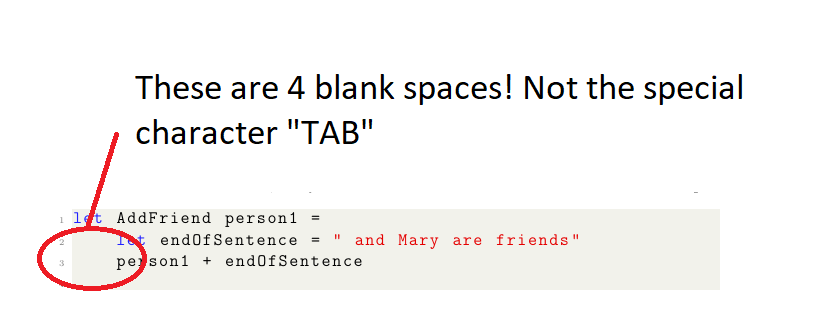
\includegraphics[width=16cm]{pictures/picture19.png}
\end{center}
If you did not configure your IDE correctly, or if you copy-and-paste the special \texttt{TAB} character from another source (e.g. Notepad), then you may see the following error:
\begin{center}
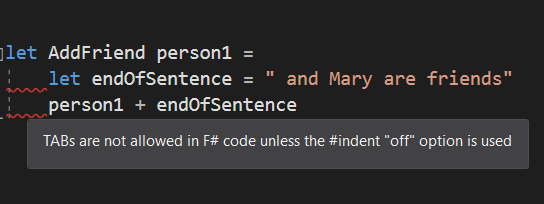
\includegraphics[width=9cm]{pictures/picture20.png}
\end{center}
\subsection{Reset F\# Interactive}
Remember to reset your F\# Interactive once in a while, so that you don't have too many previous variables (especially if you re-use the same variable names)

\begin{center}
INSERT PICTURE HERE.
\end{center}

In Visual Studio, you can Right-click the interactive window, and select ``Reset Interactive Session'', or use the shortcut key \texttt{CTRL + ALT + R}
\pagebreak

\section{Pipe-forward}
\subsection*{Key Concept:}
\begin{enumerate}
\item Coding in F\# is similar to building LEGO. 
\begin{itemize}
\item Source: \href{https://fsharpforfunandprofit.com/posts/defining-functions/}{Scott Wlaschin}
\end{itemize}
\item The output of one function is the input of the next function.
\end{enumerate}

\subsection{Introduction}
F\# has an operator, called the pipe-forward operator. 

The definition of pipe-forward is:
\begin{lstlisting}[language=FSharp]
let inline (|>) x f = f x
\end{lstlisting}
(The \texttt{inline} keyword is used to handle some special cases.) You do not need to worry about the definition. This operator is already implemented in F\# by default.

\subsection{Simple demonstration}
Let us take a look at an example:
\begin{lstlisting}[language=FSharp]
let Add5Func x = x + 5

let result1 = Add5Func 30
// val result1 : int = 35
\end{lstlisting}
Notice that the variable/input $30$ is located after the function \texttt{Add5Func}. 

However, with the new symbol \texttt{|>}, we can specify the variable/input first, and then the function that we want to apply it to.
\begin{lstlisting}[language=FSharp]
let result2 = 30 |> Add5Func
// val result2 : int = 35
\end{lstlisting}
How this code should be interpreted is the following:
\begin{center}
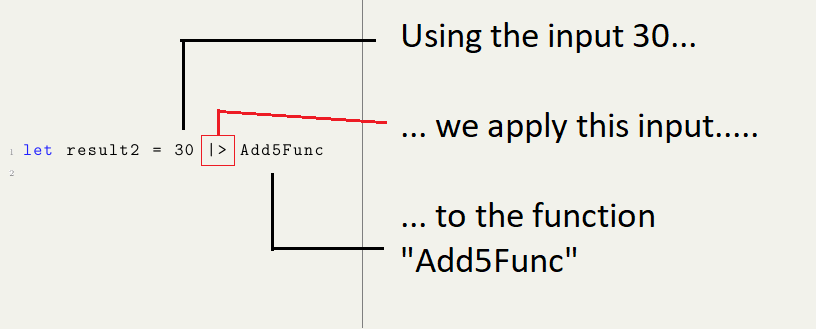
\includegraphics[width=16cm]{pictures/picture21.png}
\end{center}
\subsection{Why is this useful?}
The reason why the symbol \texttt{|>} is useful is because it helps us to compose functions. Let's say that you are given these functions:
\begin{lstlisting}[language=FSharp]
let GetGrade score =
    if score >= 90 then "A"
    else if score >= 70 then "B"
    else if score >= 50 then "C"
    else "D"

// For Singaporean University. (Maximum CAP 5.0)
let GetCAP grade =
    if grade = "A" then 5.0
    else if grade = "B" then 4.0
    else if grade = "C" then 3.0
    else 2.0
\end{lstlisting}
Remark: In American universities, they use a maximum score/GPA of $4.0$. In Singapore we use CAP  $5.0$.

We can take a look at the signatures of the functions:
\begin{lstlisting}[language=FSharp]
GetGrade: int  -> string
GetCAP:           string ->  float
\end{lstlisting}
So, we can use the result of the first function \texttt{GetGrade} as the input of a second function \texttt{GetCAP}. 
\begin{center}
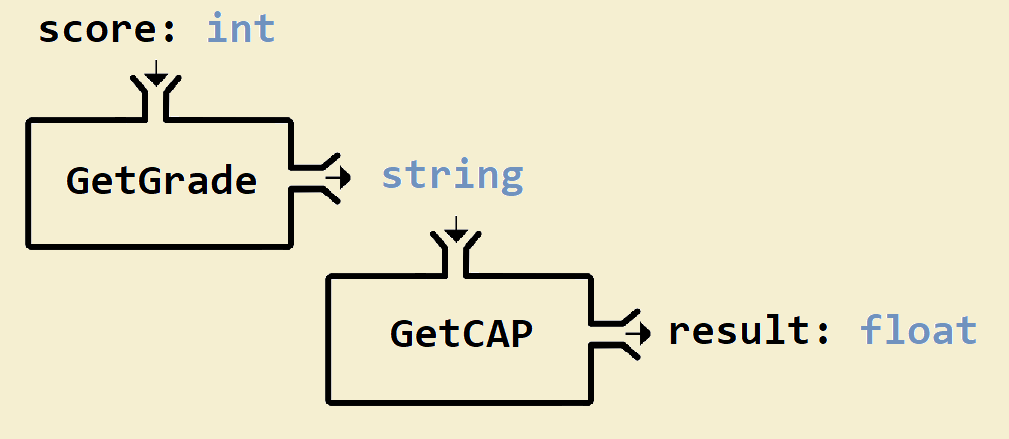
\includegraphics[width=11cm]{pictures/picture22.png}
\end{center}
\begin{lstlisting}[language=FSharp]
let GetCAPfromScore1 score =
    let intermediateResult = GetGrade score
    let finalResult = GetCAP intermediateResult
    // return
    finalResult

let cap1 = GetCAPfromScore1 95
let cap2 = GetCAPfromScore1 85
\end{lstlisting}

\pagebreak
Output:
\begin{lstlisting}[language=FSharp]
// val cap1 : float = 5.0
// val cap2 : float = 4.0
\end{lstlisting}

Notice that in the code above, we named out the intermediate steps/variables, i.e. \\\texttt{intermediateResult} and \texttt{finalResult}, even though it makes the code longer.

However, if we use the pipe-forward operator \texttt{|>}, we can simplify it as:
\begin{lstlisting}[language=FSharp]
// GetGrade: int  -> string
// GetCAP:           string ->  float
let GetCAPfromScore2 score =
    score               
    |> GetGrade         
    |> GetCAP   

let cap3 = GetCAPfromScore2 95
// val cap3 : float = 5.0
\end{lstlisting}
How this code should be interpreted:
\begin{center}
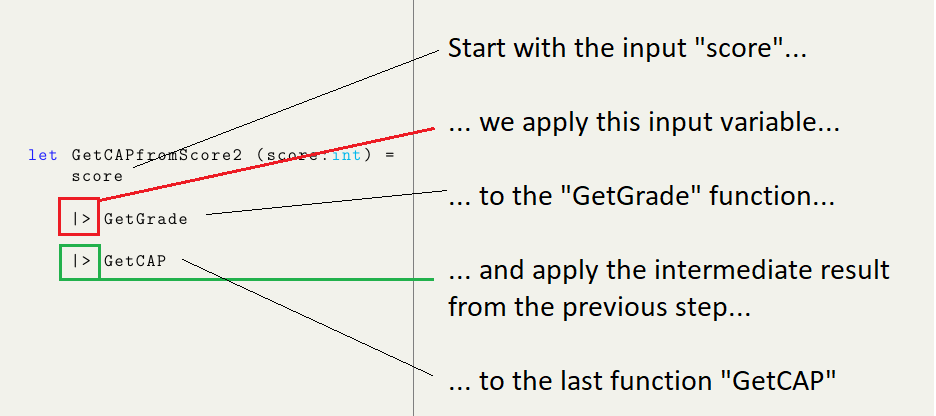
\includegraphics[width=16cm]{pictures/picture23.png}
\end{center}
Remark: The code will not compile if we put the functions in the wrong order:
\begin{lstlisting}[language=FSharp]
let CombinedFunction3Error score =
    score       // int
    |> GetCAP   // function: string -> float   // ERROR! 
    |> GetGrade // function: int -> string     // ERROR!
"ERROR!!!"
\end{lstlisting}
Because \texttt{score} is an \texttt{int}, but the function \texttt{GetCAP} only accepts  \texttt{string} as input. Similarly, the intermediate result from \texttt{GetCAP} is \texttt{float}, but the function \texttt{GetGrade} only accepts \texttt{int}
\subsection{More Examples}
Let us consider another hypothetical example. 

Imagine that you want to buy or sell a company's stock, based on the company's performance relative to the financial analyst's estimate.

\begin{enumerate}
\item F\# has a built-in function, \texttt{List.average} to find the average of a list of numbers:
\begin{lstlisting}[language=FSharp]
let average1 = List.average [1.0; 2.0; 3.0; 4.0; 5.0]
let average2 = List.average [80.0; 85.0; 90.0; 95.0; 100.0]
\end{lstlisting}
\item You are provided another function, \texttt{GetPerformance}, that determines the condition of the company.

Assume that the actual profit of the company is \$ 6.0 billion for that year, then we say that the company is:
\begin{itemize}
\item \texttt{OUTPERFORM}: If actual profit exceed the analystEstimate by 5\% 
\item \texttt{UNDERPERFORM}: If actual profit misses the analystEstimate by 5\%
\item \texttt{NEUTRAL}: If actual profit is within 5\% of the analystEstimate
\end{itemize}
\begin{lstlisting}[language=FSharp]
let GetPerformance analystAverageEstimate =
    let actualProfit = 6.0
    if actualProfit > analystAverageEstimate * 1.05
        then "OUTPERFORM"
    else if actualProfit < analystAverageEstimate * 0.95 
        then "UNDERPERFORM"
    else 
        "NEUTRAL"
\end{lstlisting}
\item You are also provided another function, \texttt{GetNumSharesToBuy}, that determines how much additional shares to buy/sell depending on the company's condition:

\begin{itemize}
\item \texttt{OUTPERFORM}: Buy additional $1000$ shares.
\item \texttt{UNDERPERFORM}: Sell $1000$ shares.
\item \texttt{NEUTRAL}: Hold the same portfolio.
\end{itemize}
\begin{lstlisting}[language=FSharp]
let GetNumSharesToBuy performance =
    if performance = "OUTPERFORM" then
        1000     // buy 1000 shares
    else if performance = "UNDERPERFORM" then
        -1000    // sell 1000 shares
    else 
        0       // hold.
\end{lstlisting}
\end{enumerate}
So, the function signatures are:
\begin{lstlisting}[language=FSharp]
List.average:        
    List<double> -> double
GetPerformance:     double -> string
GetNumSharesToBuy:            string -> int
\end{lstlisting}
In this carefully crafted example, notice that the result of the one function can act as the input to the other function. 
\begin{center}
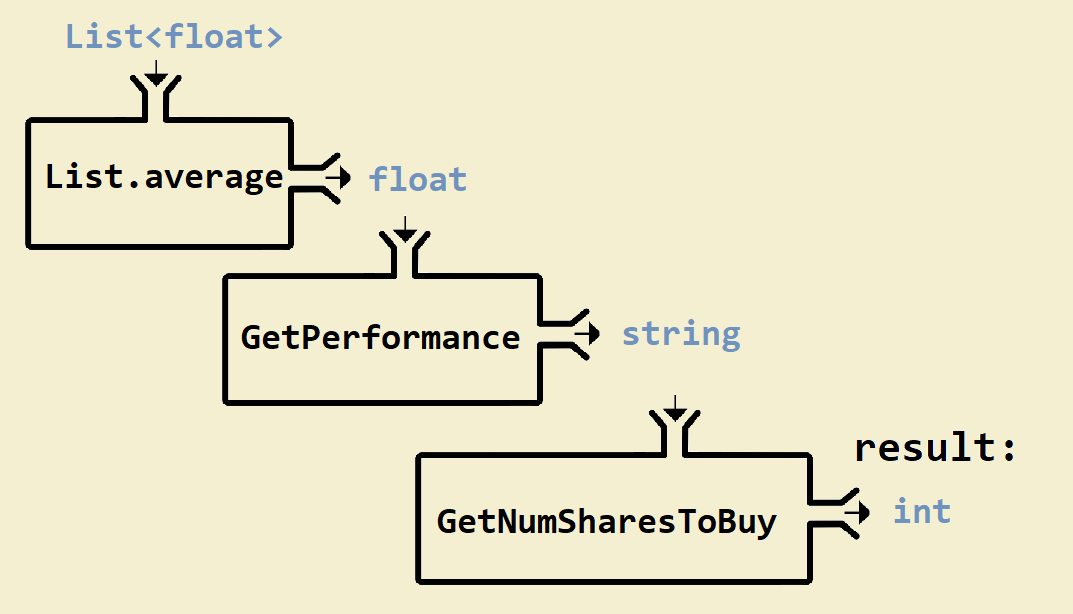
\includegraphics[width=16cm]{pictures/picture24.png}
\end{center}
So, we can combine them into a big function:
\begin{lstlisting}[language=FSharp]
// Assume the profit is already known to be $6.0 billion, and written in "GetPerformance"
let GetNumSharesFromEstimate1 individualEstimates =
    let intermediateResult1 = 
        List.average individualEstimates

    let intermediateResult2 = 
        GetPerformance intermediateResult1

    let finalResult = GetNumSharesToBuy intermediateResult2
    // output
    finalResult
\end{lstlisting}
Notice that the code above uses a lot of temporary variables \texttt{intermediateResult1}, etc. which makes the code unnecessarily longer.

\pagebreak

Usage example:
\begin{enumerate}
\item In this example, the actual profit (6.0 billion) exceeds all the financial analyst's prediction, which means this is good news.
\begin{lstlisting}[language=FSharp]
let numShares1 = GetNumSharesFromEstimate1 [4.0; 5.0; 3.0; 2.0; 2.5]
printfn "Number of shares to buy(+) or sell(-): %i" numShares1
// Output:
// "Number of shares to buy(+) or sell(-): 1000"
\end{lstlisting}
\item In this example, the actual profit (6.0 billion) misses all the financial analyst's prediction, which means this is bad news.
\begin{lstlisting}[language=FSharp]
let numShares2 = GetNumSharesFromEstimate1 [8.0; 7.0; 10.0; 12.0; 10.5]
printfn "Number of shares to buy(+) or sell(-): %i" numShares2
// Output:
// "Number of shares to buy(+) or sell(-): -1000"
\end{lstlisting}
\end{enumerate}
The following is the original code:
\begin{lstlisting}[language=FSharp]
// Assume the profit is already known to be $6.0 billion, and written in "GetPerformance"
let GetNumSharesFromEstimate1 individualEstimates =
    let intermediateResult1 = 
        List.average individualEstimates
    let intermediateResult2 = 
        GetPerformance intermediateResult1
    let finalResult = GetNumSharesToBuy intermediateResult2
    // output
    finalResult
\end{lstlisting}
And the following is the simplified version with the pipe-forward operator \texttt{|>}

\begin{lstlisting}[language=FSharp]
let GetNumSharesFromEstimate2 individualEstimates =
    individualEstimates                 
    |> List.average                     
    |> GetPerformance                  
    |> GetNumSharesToBuy  
\end{lstlisting}

How this code should be interpreted:
\begin{center}
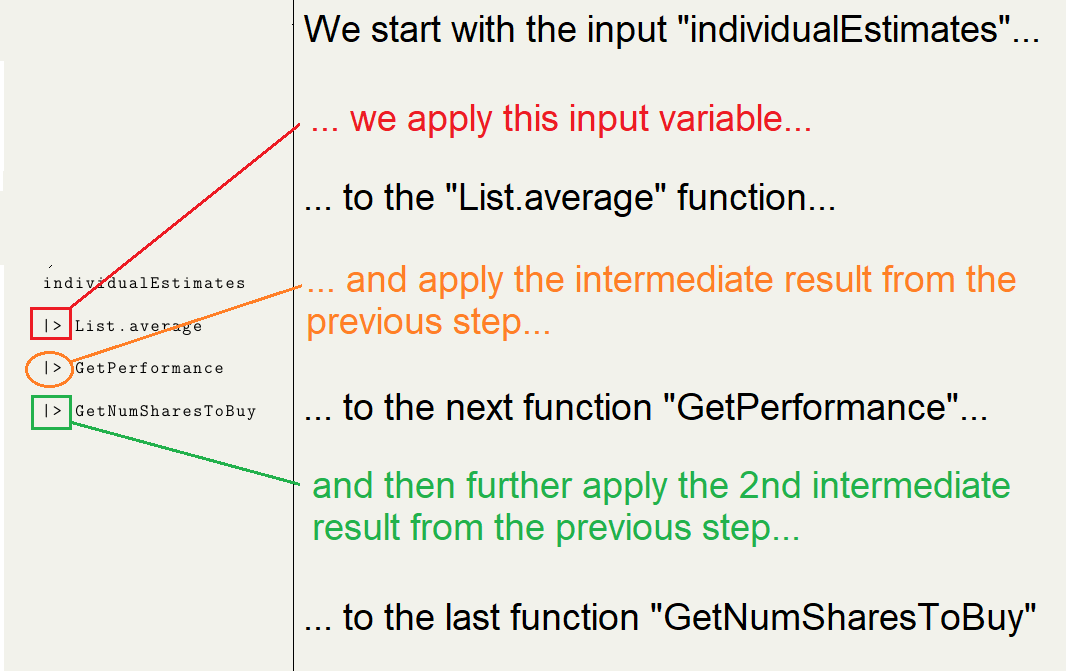
\includegraphics[width=14cm]{pictures/picture25.png}
\end{center}   

\subsection{Benefits}
The benefits of using the pipe-forward operator \texttt{|>}:
\begin{enumerate}
\item You can remove unnecessary clutter/words on our computer screen. You do not need explicitly write out intermediate result, and we can focus more on the internal logic/calculations (and reserve the naming for variables/results that are truely important).

\item It is easier to follow instructions than to reason mathematically. Consider the following two statements:
\[
 y = h\left(g \left(f \left(x \right)\right)\right)
\]
\begin{lstlisting}
Start with variable x.
Step 1: Use function f.
Step 2: Use function g.
Step 3: Use function h.
\end{lstlisting}
Most common languages* are written from left-to-right, and top-to-bottom. So, the conventional mathematical notation $h\left(g \left(f \left(x \right)\right)\right)$ is not very natural to most languages. Whereas in the second case, it gives us a simple step-by-step instructions on how to get our final result. 

This makes it easier to non-programmers to understand your code (e.g. if you work with a manager or a trader); it makes it easier for you to understand your own code (e.g. if you re-visit some code that you have written 1 year ago). 

*Exception: Hebrew and Arabic.

\end{enumerate}
Once you get used to this syntax, you may find other traditional programming language, e.g. Java/ C++ to be a bit verbose/too long.

\pagebreak

\subsection{Intellisense}
In actual code development, we will do things step by step (instead of collecting everything together and chain everything using \texttt{|>}). 

\begin{enumerate}
\item We will first start off like this:
\begin{lstlisting}[language=FSharp]
let myFunction1 (individualEstimates: List<float>) =
    individualEstimates                 
    |> List.average     

  
\end{lstlisting}
If you are using VisualStudio or VisualStudioCode, hover your mouse over \texttt{myFunction1} to see the type signature:
\begin{lstlisting}[language=FSharp]
List<float> -> float
\end{lstlisting}
\item Next, let's add one more line:
\begin{lstlisting}[language=FSharp]
let myFunction2 individualEstimates =
    individualEstimates                 
    |> List.average                     
    |> GetPerformance         
\end{lstlisting}
We know that until the \texttt{List.average} step, we have an intermediate result of type \texttt{float}. So, we want the next function, \texttt{GetPerformance}, to take in \texttt{float} as an input. 

Hover your mouse over \texttt{myFunction2} to see the type signature:
\begin{lstlisting}[language=FSharp]
List<float>          -> string
\end{lstlisting}
\item Finally, let's add one more line:
\begin{lstlisting}[language=FSharp]
let myFunction3 individualEstimates =
    individualEstimates                 
    |> List.average                     
    |> GetPerformance                
    |> GetNumSharesToBuy     
\end{lstlisting}
The new function, \texttt{GetNumSharesToBuy}, should ideally accept \texttt{string} as its input (which it does). And if we hover your mouse over \texttt{myFunction3} to see the type signature:
\begin{lstlisting}[language=FSharp]
List<float>                    -> int
\end{lstlisting}
\end{enumerate}

\pagebreak
\subsection{Exercise}
Scenario: Assume that you are in a trading firm, and you want to manage your employees based on their performance.

You are given the following functions:
\begin{enumerate}
\item The F\# build-in function, \texttt{List.sum} that finds the sum of a list of doubles/decimals.
\begin{lstlisting}[language=FSharp]
let sum1 = List.sum [1.0; 2.0; 3.0; 4.0; 5.0]   // sum from 1 to 5
let sum2 = List.sum [1.0 .. 100.0]              // sum from 1 to 100
\end{lstlisting}
\item Another function, \texttt{GetStatus}, that determines how well is the trader
\begin{itemize}
\item \texttt{TOP TRADER}: Profit exceeds \$ 10.0 million.
\item \texttt{HUGE LOSSES}: Loses \$3.0 million.
\item \texttt{NORMAL TRADER}: Remaining cases
\end{itemize}
\begin{lstlisting}[language=FSharp]
let GetStatus profit =
    if profit > 10.0 then
        "TOP TRADER"
    else if profit < -3.0 then
        "HUGE LOSSES"
    else
        "NORMAL TRADER"
\end{lstlisting}
\item Another function, \texttt{GetBonus}, that determines how many months of bonus is given to the trader.
\begin{itemize}
\item \texttt{TOP TRADER}: 24 months bonus (i.e. 2 years bonus)
\item \texttt{HUGE LOSSES}: 6 months bonus (i.e. half year bonus)
\item \texttt{NORMAL TRADER}: 0 months bonus (i.e. no bonus)
\end{itemize}
\begin{lstlisting}[language=FSharp]
let GetBonus status =
    if status = "TOP TRADER" then   
        24      // 24-month, i.e. 2 year bonus.
    else if status = "NORMAL TRADER" then
        6       // 6-month, i.e. half year bonus.
    else 
        0       // No bonus.
\end{lstlisting}
\pagebreak
\end{enumerate}
Again, the output of one function is the input of the next function:
\begin{lstlisting}[language=FSharp]
List.sum : List<double> -> double
GetStatus:                 double -> string
GetBonus:                            string -> int
\end{lstlisting}

\begin{lstlisting}[language=FSharp]
let GetBonusFromTrades1 listOfTrades =
    let intermediateResult1 = List.sum listOfTrades
    let intermediateResult2 = GetStatus intermediateResult1
    let finalResult = GetBonus intermediateResult2
    // output
    finalResult
\end{lstlisting}

Try to re-implement the function above using the pipe-forward operator \texttt{|>}.
\begin{lstlisting}[language=FSharp]
let GetBonusFromTrades2 (listOfTrades: List<double>) =










    // implement the function above.
\end{lstlisting}

\vspace{1.0cm}

Examples of use cases:
\begin{enumerate}
\item This trader helped the company earned some money. 
\begin{lstlisting}[language=FSharp]
let bonus1 = 
    GetBonusFromTrades2 [1.0; -2.0; 0.5; 0.3; 0.4; 0.2]
printfn "He received a bonus of %i months" bonus1
\end{lstlisting}
\item This trader made one huge profitable deal, with other tiny losses.

\begin{lstlisting}[language=FSharp]
let bonus2 = 
    GetBonusFromTrades2 [-2.0; -1.0; -0.5; 30.0; -1.0]
printfn "She received a bonus of %i months" bonus2
\end{lstlisting}
\end{enumerate}

\subsection{Function with same input and output type}
The mathematical term is called \textit{endomorphism}. 

In all the above examples, we have chosen functions that have different input and output types, so that it is obvious which function comes after which one.

Sometimes, you may face with functions that have the same input and output type. For example:
\begin{lstlisting}[language=FSharp]
let Square x = x * x
let Cube x = x * x * x
let Add5 x = x + 5

// Square: int -> int
// Cube  : int -> int
// Add5  : int -> int
\end{lstlisting}
All of these functions are \texttt{int -> int}, and so you may compose them in different orders, or you may apply the same function multiple times, which may cause the function to completely change.
\begin{enumerate}
\item Example 1
\[
f_1(x) = \left(x^2 + 5\right)^3
\]
\begin{lstlisting}[language=FSharp]
let f1 x = 
    x
    |> Square
    |> Add5
    |> Cube
    
// (1^2 + 5) ^ 3 = 216
let demo1 = f1 1

// (2^2 + 5) ^ 3 = 729
let demo2 = f1 2
\end{lstlisting}
Output:
\begin{lstlisting}[language=FSharp]
// val demo1 : int = 216
// val demo2 : int = 729
\end{lstlisting}

\pagebreak
\item Example 2
\[
f_2(x) = \left(x^2\right)^3 + 5
\]
\begin{lstlisting}[language=FSharp]
let f2 x =
    x
    |> Square
    |> Cube
    |> Add5
    
// (1^2)^3 + 5 = 6
let demo3 = f2 1

// (2^2)^3 + 5 = 71
let demo4 = f2 2
\end{lstlisting}
Output:
\begin{lstlisting}[language=FSharp]
// val demo3 : int = 6
// val demo4 : int = 69
\end{lstlisting}
\item Exercise:

Try to implement the following function using pipe-forward:
\[
f_3(x) = \left[\left(x + 5\right)^2 + 5\right]^3
\]
\begin{lstlisting}[language=FSharp]
//let Square x = x * x
//let Cube x = x * x * x
//let Add5 x = x + 5
let f3 x =





	// IMPLEMENT YOUR FUNCTION ABOVE

// Testing:
// [   (1+5)^2   + 5   ]^3 = 68921
let demo5 = f3 1

// [   (2+5)^2   + 5   ]^3 = 157464
let demo6 = f3 2
\end{lstlisting}
\end{enumerate}

\pagebreak

\section{List in F\#}
Key Concept:
\begin{enumerate}
\item Introduce basic \texttt{List} functions
\begin{enumerate}
\item \texttt{List.filter} 
\item \texttt{List.map}
\end{enumerate}
\item Code in F\# are very easy to understand (thanks for pipe-forward operator \texttt{|>} and the F\# language design)
\item Anonymous functions / lambda function also helps.
\begin{itemize}
\item You are defining a function at the exact location where it is most useful. So it boosts productivity.
\item \texttt{fun} is a keyword in F\#! 
\end{itemize}
\end{enumerate}

\subsection{Creating a list}
You can create a list of integers/ float / string using the following notations:
\begin{lstlisting}[language=FSharp]
let list1 = [1 .. 100]          
let list2 = [50 .. 80]
let list3 = [1 .. 2 .. 100]      

let list4 = [1.0 .. 100.0]      
let list5 = [0.0 .. 0.05 .. 1.0]

let list6 = [1; 20; 50; 100; 55; 5; 10]
let list7 = [1.0; 6.0; 5.0; 10.0; 3.0; 2.0]

let list8 = ["ABC";"DEF";"GHI";"JKL";"MNO"]
\end{lstlisting}
The \texttt{;} is used to separate different elements, and \texttt{[a .. b], [a .. diff .. b]} is used to specify any increasing/decreasing pattern.

If you hover your mouse on top of those variables (using VisualStudio or VisualStudioCode), you will see the types are \texttt{int list, float list, etc.} An alternate notation would be \texttt{List<int>, List<double>, etc.}

Warning: You cannot create a list with different types, e.g. the example below tries to create a list with a string, an integer, and a decimal/float.
\begin{lstlisting}[language=FSharp]
let listError = ["ABC"; 123; 400.0]
// ERROR! Cannot define different type in the same list!
\end{lstlisting}

\pagebreak

\subsection{\texttt{List.filter}}
Here is a simple function that returns true/false, depending on whether $x$ is divisible by $2$:
\begin{lstlisting}[language=FSharp]
let IsItEven x = (x % 2 = 0)

let trueOrFalse1 = IsItEven 10
let trueOrFalse2 = IsItEven 3
\end{lstlisting}
Remark: \texttt{x \% 2} means the remainder after we divide $x$ by $2$.

We can use this function together with \texttt{List.filter}:
\begin{lstlisting}[language=FSharp]
let result1 = List.filter IsItEven [1 .. 100]
// Output:
// [2; 4; 6; ......; 98; 100]
\end{lstlisting}
The \texttt{List.filter} function filters a list, and only select the elements which satisfy some requirement; the requirement is specified through a function \texttt{IsItEven}.

Alternatively, because the definition of \texttt{IsItEven} is quite easy, we can even implement it immediately after \texttt{List.filter}, at the point where we need it the most.
\begin{lstlisting}[language=FSharp]
let result2 = List.filter (fun x -> x % 2 = 0) [1 .. 100]
// Output:
// [2; 4; 6; ......; 98; 100]
\end{lstlisting}
The notation \texttt{(fun x -> x \% 2 = 0)} is used to define anonymous/lambda function, i.e. functions that are easy to define, that we do not need to give it a name, e.g. \texttt{IsItEven}.

Benefits:
\begin{itemize}
\item We define this function using the \texttt{fun} keyword at exactly where it is used.
\item If we define too many custom functions, e.g. \texttt{IsItEven}, then it will be hard to keep track when we have 1000+ functions, and we will lose productivity.
\end{itemize}
Remark: The code \texttt{(fun x -> x \% 2 = 0)} represents a ``thing'', and that ``thing'' is a \underline{function}, just like \texttt{IsItEven} is a function.

Side note: \texttt{fun} is a keyword in the F\#! Programming in F\# is very fun!

\pagebreak
\subsubsection*{\texttt{List.filter} and Pipe-Forward \texttt{|>}}
Let us look at the following function:
\begin{lstlisting}[language=FSharp]
let SumMultiplesOfThree xList =
    xList
    |> List.filter (fun x -> x % 3 = 0)
    |> List.sum
\end{lstlisting}
How to interpret this function:
\begin{center}
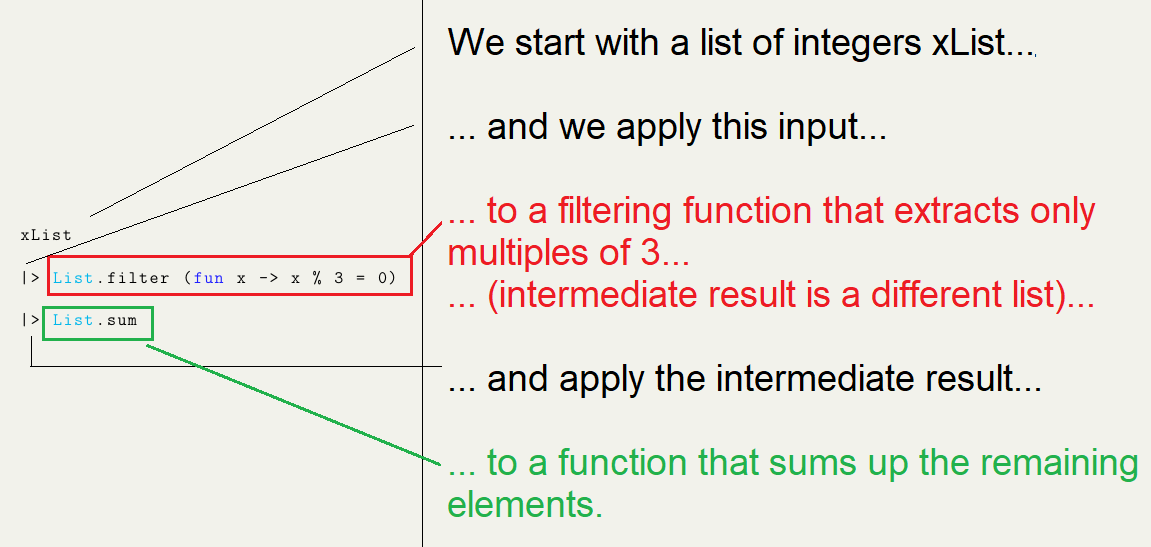
\includegraphics[width=16cm]{pictures/picture26.png}
\end{center}
So, F\# is able to express all of these calculations with just 3 lines of code, which is quite elegant, maybe similar to Python code (in style), compared to other more traditional languages (Java/C++) which we need to write longer.

Using this function:
\begin{lstlisting}[language=FSharp]
// 3 + 6 + 9 + ... + 99 = 1683
let result3 = SumMultiplesOfThree [1 .. 100]

// 3 + 6 + 9 + ... + 198 = 6633
let result4 = SumMultiplesOfThree [1 .. 200]
\end{lstlisting}
Output:
\begin{lstlisting}[language=FSharp]
// val result3 : int = 1683
// val result4 : int = 6633
\end{lstlisting}

\pagebreak
\subsubsection*{Another example}
Let's say you want to find out how many students in your class got at least $80$ points in an exam.
\begin{lstlisting}[language=FSharp]
let CountGreaterThan80 scoreList =
    scoreList
    |> List.filter (fun x -> x >= 80)
    |> List.length
\end{lstlisting}
How to interpret this function:
\begin{center}
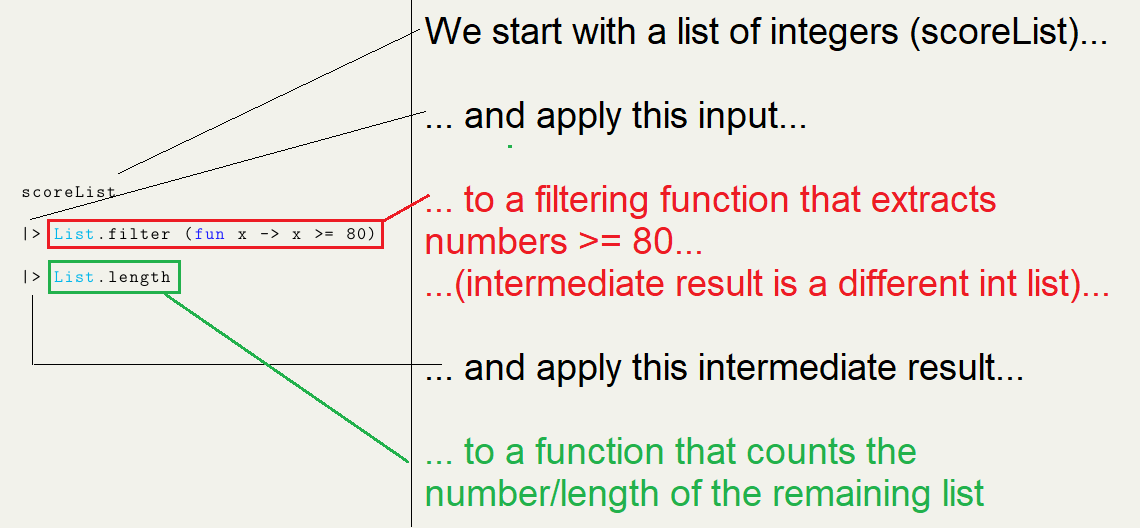
\includegraphics[width=16cm]{pictures/picture27.png}
\end{center}
Using this function:
\begin{lstlisting}[language=FSharp]
let result5 = 
    CountGreaterThan80 [60; 65; 70; 75; 80; 85; 90; 95]
printfn "%i students scored 80 or above." result5
\end{lstlisting}
Output:
\begin{lstlisting}[language=FSharp]
// "4 students scored 80 or above."
\end{lstlisting}

\pagebreak
\subsubsection*{Another example}
This function adds up all multiples of $3$, e.g. $3, 6, 9, \ldots$, but ignore all multiples of $5$,
\\ e.g. $5, 10, \underline{\mathbf{15}}, 20, 25, \underline{\mathbf{30}}, \ldots$
\begin{lstlisting}[language=FSharp]
let SumMultiplesOf3ButNot5 xList =
    xList
    |> List.filter (fun x -> (x % 3 = 0) && (x % 5 <> 0))
    |> List.sum

let result6 = SumMultiplesOf3ButNot5 [1 .. 100]
\end{lstlisting}
Output: 
\begin{lstlisting}[language=FSharp]
// val result6 : int = 1368
\end{lstlisting}
Remark:
\begin{itemize}
\item \texttt{(x \% 3 = 0)}: is x divisible by 3?
\item \texttt{(x \% 5 <> 0)}: is x NOT a multiple of 5?
\end{itemize}

\subsubsection*{Exercise}
Implement a function that sums up all multiples of $3$ or $5$ in a list.

\begin{lstlisting}[language=FSharp]
let SumMultiplesOf3Or5 xList =




    // Hint:  || means OR, && means AND

// From 1 to 10, the multiples of 3 or 5 are 3, 5, 6, 9, 10
// 3 + 5 + 6 + 9 + 10 = 33
let result7 = SumMultiplesOf3Or5 [1 .. 10]

let result8 = SumMultiplesOf3Or5 [1 .. 999]
\end{lstlisting}

Remark: After you have completed this question, you can create an account an submit your solution here for personal achievement/accomplishment.

\url{https://projecteuler.net/problem=1}

\pagebreak

\subsection{\texttt{List.map}}

\begin{lstlisting}[language=FSharp]
let Square x = x * x
let result9 = List.map Square [1 .. 10]
\end{lstlisting}
The \texttt{List.map} function transform each individual element of a list using some transformation. The transformation is specified through a function \texttt{Square}.
\begin{center}
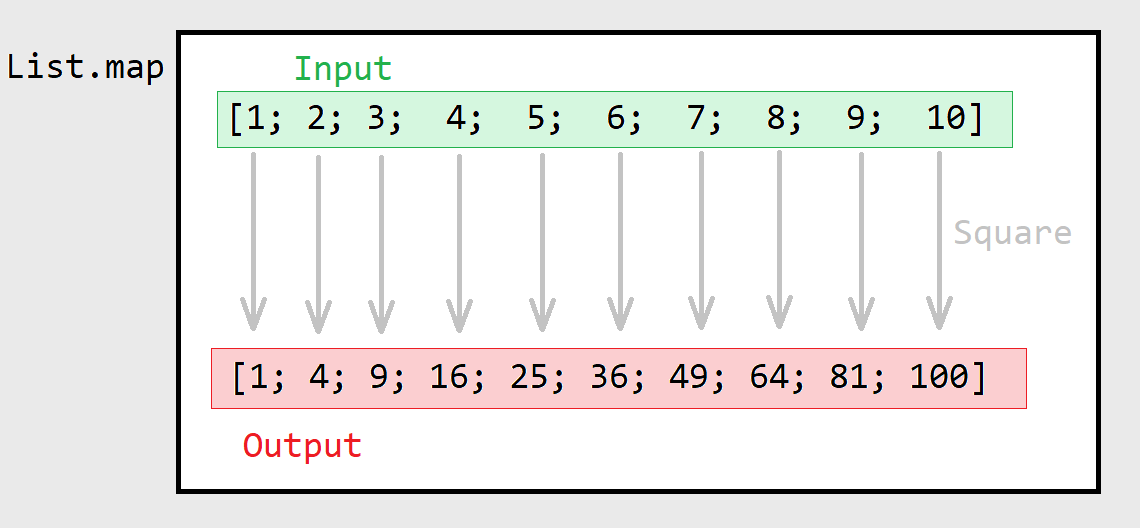
\includegraphics[width=10cm]{pictures/picture28.png}
\end{center}   
Alternatively, we can use the \texttt{fun} keyword to define the \texttt{Square} function
\begin{lstlisting}[language=FSharp]
let result10 = List.map (fun x -> x * x) [1 .. 100]
\end{lstlisting}
\subsubsection*{\texttt{List.map} and Pipe-Forward \texttt{|>}}
Let us look at an example:

\begin{lstlisting}[language=FSharp]
let SumOfSquares xList =
    xList
    |> List.map (fun x -> x * x)
    |> List.sum

// 1^2 + 2^2 + 3^2 + 4^2 + ... + 10^2 = 385
let result11 = SumOfSquares [1 .. 10]
\end{lstlisting}
How to interpret the code:
\begin{center}
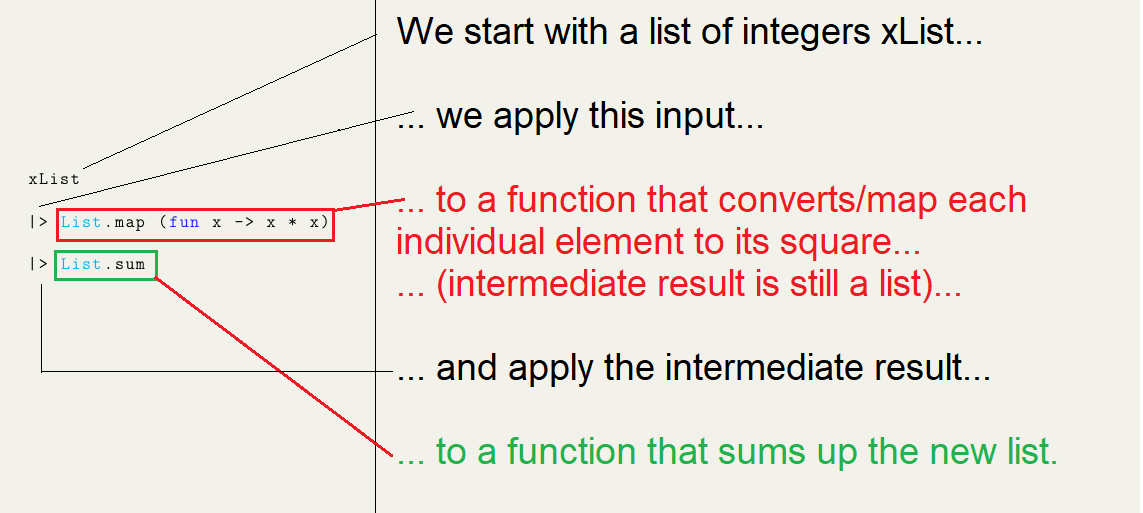
\includegraphics[width=14cm]{pictures/picture29.png}
\end{center}

\pagebreak
\subsubsection*{Exercise}
There are two supermarkets in town. One of them want to round the prices of each \underline{individual} goods to the nearest dollar (might round-up or round-down). The other want to round DOWN the prices of each individual goods to the nearest dollar.

The functions \texttt{System.Math.Floor, System.Math.Round}* are used round the prices:
\begin{lstlisting}[language=FSharp]
let originalPrice1 = 1.35
let originalPrice2 = 3.99

let newPrice1 = originalPrice1 |> System.Math.Floor
let newPrice2 = originalPrice2 |> System.Math.Floor

// Temporary ignore decimal numbers like 1.50, 2.50.
let newPrice3 = originalPrice1 |> System.Math.Round
let newPrice4 = originalPrice2 |> System.Math.Round
\end{lstlisting}

Output:
\begin{lstlisting}[language=FSharp]
val newPrice1 : float = 1.0
val newPrice2 : float = 3.0

val newPrice3 : float = 1.0
val newPrice4 : float = 4.0
\end{lstlisting}
*Remark: We will temporary ignore decimals like $1.50, 2.50$, because F\# uses ``Banker's Rounding'' when tie-breaking is required. (Google it for more info)
\begin{enumerate}
\item Write a function that accepts a list of prices of the original products, and computes the final price of everything after each item are individually rounded-down.
\begin{lstlisting}[language=FSharp]
// Round the prices to closest integer (ignore 1.50, 2.50, etc.)
let TotalPriceAfterRoundDown priceList =



     // Implement your function here.
\end{lstlisting}

\item Write a function that accepts a list of prices of the original products, and computes the final price of everything after each item are individually rounded to the nearest integer (ignore $1.50, 2.50,$ etc.).
\begin{lstlisting}[language=FSharp]
let TotalPriceAfterRound priceList =



     // Implement your function here.
\end{lstlisting}
\end{enumerate}

\pagebreak

\subsubsection*{Application: Sample Variance}
We will try to implement the sample variance function (\texttt{VAR.S} in Excel 2010 or later, or see \url{https://www.miniwebtool.com/sample-variance-calculator/}).
\[
\text{Sample Variance} = \dfrac{1}{N - 1} \sum_{i=1}^N \left(x_i - \overline{x}\right)^2
\]
Remark: It is divided by $N-1$, not $N$, because of statistics reasons (Bessel's correction).
\begin{lstlisting}[language=FSharp]
let SampleVariance xList =
    let N = 
        xList
        |> List.length
        |> double         // The "double" function 

    let average = 
        xList
        |> List.average

    // return this:
    xList
    |> List.map (fun x -> (x - average) ** 2.0)
    |> List.sum
    |> fun final -> final / (N - 1.0)       
\end{lstlisting}
Remark:
\begin{enumerate}
\item We use the \texttt{double} function to convert an integer to decimal (you can also use it to process \texttt{string} to decimals, if the \texttt{string} is well defined)
\item At the last step, we divide by \texttt{(N - 1.0)} and not \texttt{(N - 1)} because we are working with decimals.
\item The compiler knows xList is a \texttt{float list} or \texttt{List<float>}, because at some point it interacted with \texttt{** 2.0}. 
\end{enumerate}
\begin{lstlisting}[language=FSharp]
let result12 = SampleVariance [1.0 .. 7.0]      
// val result12 : double = 4.666666667
\end{lstlisting}

\pagebreak

\subsubsection*{Exercise}
Given a list of integers $x_1, x_2, \ldots, x_n$, write a function that calculates the following:
\[
\left(\sum_{i=1}^n x_i\right)^2 - \left(\sum_{i=1}^n {x_i}^2\right)
\]
If you want, you can use the following hint:
\begin{lstlisting}[language=FSharp]
let ProjectEulerProblem6 xList =
    // if xList = [a;b;c], calculate a^2 + b^2 + c^2
    let sumOfSquares = 




    // if xList = [a;b;c], calculate a + b + c
    let sum =




    // return
    (sum * sum) - sumOfSquares
\end{lstlisting}

To use the function:
\begin{lstlisting}[language=FSharp]
let result13 = ProjectEulerProblem6 [1 .. 100]
printfn "Answer for ProjectEuler Problem6 is: %i" result13
\end{lstlisting}
Remark: After you have completed this question, you can create an account an submit your solution here for personal achievement/accomplishment.

\url{https://projecteuler.net/problem=6}

\subsubsection*{Exercise}
You are given the following function that determines whether a positive integer \texttt{x} is a prime number or not. You can just directly use it. You do not need to implement it yourself.
\begin{lstlisting}[language=FSharp]
let IsPrime x =
    let squareRoot = x |> double |> sqrt |> int 
    if x = 1 then false
    else if x = 2 then true
    else if x % 2 = 0 then false
    else 
        [3 .. 2 .. squareRoot]
        |> List.forall (fun i -> x%i <> 0)

// val IsPrime: x:int -> bool
\end{lstlisting}
Reminder: You can directly use the \texttt{IsPrime} function in the previous page. You do not need to re-implement it again.

Write a function that takes in a list of positive integers, and sums all the prime numbers.
\begin{lstlisting}[language=FSharp]
let Problem10_Version1 (xList: List<int>) =






// test:
let result1 = Problem10_Version1 [1 .. 9]
// 2 + 3 + 5 + 7 = 17.

let result2 = Problem10_Version1 [1 .. 99]
// 2 + 3 + 5 + 7 + 11 + ... + 83 + 89 + 97 = 1060.
\end{lstlisting}
However, if you try the following, you may potentially encounter an error:
\begin{lstlisting}[language=FSharp]
let result3 = Problem10_Version1 [2 .. 2000000]
// ERROR!
// System.OverflowException: Arithmetic operation resulted in an overflow.
\end{lstlisting}
This is because there are too many numbers to sum up, and the \texttt{int} datatype cannot handle large sums.

A workaround is to use the \texttt{System.Numerics.BigInteger} (Java also has such BigInteger standard library). We convert each individual prime number into a \texttt{BigInteger} before sum them all up.

\begin{lstlisting}[language=FSharp]
open System.Numerics

let SumAllPrimes xList =
    xList
    |> List.filter (IsPrime)
    |> List.map (BigInteger)
    |> List.sum

// Remark: The code below can take 10 seconds, as this is not the most optimal algorithm.
let result17 = SumAllPrimes [2 .. 2000000]
printfn "The sum of all primes from 2 to 2000000 is: %A" result17
\end{lstlisting}
Remark: After you have completed this question, you can create an account an submit your solution here for personal achievement/accomplishment.

\url{https://projecteuler.net/problem=10}

\pagebreak

\subsubsection*{Optional Exercise (Try this at home)}
\url{https://projecteuler.net/problem=3}

Given an integer $Z$, write a function that finds the largest prime factor of $Z$. e.g. The prime factors of $13195$ are $5, 7, 13, 29$, and so the largest for $13195$ is $29$.

\subsubsection*{Problem Analysis}
To find the largest prime factor for $Z$, we will first try to find all factors of $Z$ (not necessarily prime factors) between $1$ and $\sqrt{Z}$. 

Let $S_1 = \{a_1, \ldots, a_n\}$ be all the factors of $Z$ (not necessarily prime factors) between $1$ and $\sqrt{Z}$. This set will always contain at least one element: $a_1 = 1$.

Let $S_2 = \left\{\dfrac{Z}{a_1},\ldots, \dfrac{Z}{a_n}\right\}$. These are all the factors of $Z$ between $\sqrt{Z}$ and $Z$. This set will always contain at least one element: $\dfrac{Z}{a_1} = Z$.

And so, $S_1 \cup S_2 =  \left\{a_1, \ldots, a_n, \dfrac{Z}{a_1},\ldots, \dfrac{Z}{a_n}\right\}$ are all the factor of $Z$ (not necessarily prime factors). And we just need to find that out of this set $S_1 \cup S_2$, which number is the largest \underline{prime} number.

\begin{enumerate}
\item Example: $3 \times 7 = 21$. The largest prime factor is $7 > \sqrt{21} \approx 4.58$.

\item Example: $6 \times 11 = 66$. The largest prime factor is $11 > \sqrt{66} \approx 8.12$.
\end{enumerate}

\subsubsection*{Hints:}
\begin{enumerate}
\item The function \texttt{IsPrimeBigInteger} is implemented for you. This is a slightly modified version of the \texttt{IsPrime} function that takes in a \texttt{BigInteger} as an input (as compared to an \texttt{int}). No need to re-implement this function.

\begin{lstlisting}[language=FSharp]
let IsPrimeBigInteger x =
    let squareRoot = x |> double |> sqrt |> BigInteger 
    if x = BigInteger(1) then false
    else if x = BigInteger(2) then true
    else if x % BigInteger(2) = BigInteger(0) then false
    else 
        [BigInteger(3) .. BigInteger(2) .. squareRoot]
        |> List.forall (fun i -> x%i <> BigInteger(0))
\end{lstlisting}
\item To determine whether \texttt{x} is divisible by \texttt{y}, when \texttt{x, y} are both \texttt{BigInteger}s, do the following:
\begin{lstlisting}[language=FSharp]
x % y = BigInteger(0)
\end{lstlisting}
We cannot do \texttt{x \% y = 0}, because we cannot \underline{directly} compare a \texttt{BigInteger} with an integer.
\end{enumerate}
\begin{lstlisting}[language=FSharp]
open System.Numerics

let FindLargestPrimeFactor (Z: BigInteger) =
    let approxSqrt = Z |> double |> sqrt |> BigInteger

    // Find factors of Z between [2 .. sqrt(Z)]
    // Not necessarily prime factors.
    let list1 =
        [BigInteger(2) .. approxSqrt]
        |> ......

        // Complete the logic above

    // Produce another list such that:
    // For each element "a" in list1, it gives "Z / a"
    let list2 =
        list1
        |> ......

        // Complete the logic above

    // List.append combines the two lists.
    let combinedList =
        List.append list1 list2

    // Choose only prime numbers from the combinedList, and find the maximum using List.max
    combinedList
    |> ......

    // Complete the logic above
\end{lstlisting}
\begin{lstlisting}[language=FSharp]
let number1 = BigInteger(21)
let result18 = FindLargestPrimeFactor number1  
// Expect result: 7

let number2 = BigInteger(66)
let result19 = FindLargestPrimeFactor number2
// Expect result: 11

let number3 = BigInteger.Parse("600851475143")
let result20 = FindLargestPrimeFactor number3
\end{lstlisting}

Remark: After you have completed this question, you can create an account an submit your solution online for personal achievement/accomplishment.
\pagebreak

\section{Tuples, Records, Discriminated Union}
Key concept:
\begin{enumerate}
\item Tuple is a good data-structure for many things:
\begin{enumerate}
\item To represents terms that goes together, e.g. 2-D coordinates, Year-Month, etc.
\item For pattern matching, especially for pairwise operation or grouping operation.
\item For testing out ideas quickly. (and use other data-structures after you have done testing)
\end{enumerate} 
\item You can directly extract the content of a tuple, and use underscore ``\underline{\:\:}'' to ignore any part of the tuple that you don't need.
\end{enumerate}

\subsection{Tuples}
A 2D-coordinate may look like this:
\begin{lstlisting}[language=FSharp]
let point1 = (1.0, 2.0)
let point2 = (3.0, 4.0)
\end{lstlisting}
Hover your mouse on top of these two objects. Notice that the signature is \texttt{float * float}. So these points have two coordinates, each of them are \texttt{float} or \texttt{double}

\begin{lstlisting}[language=FSharp]
let DistanceFromOrigin point =
    let (x,y) = point        // Data extraction process!
    sqrt (x ** 2.0 + y ** 2.0)

let distance1 = DistanceFromOrigin point1
printfn "The first point is distance %f away from origin" distance1

let distance2 = DistanceFromOrigin point2
printfn "The second point is distance %f away from origin" distance2
\end{lstlisting}
Output:
\begin{lstlisting}[language=FSharp]
// The first point is distance 2.236068 away from origin
// The second point is distance 5.000000 away from origin
\end{lstlisting}
Notice that we have an extraction process \texttt{let (x,y) = point} that helps us extract the contents of \texttt{point} (and save the contents into the variables \texttt{x,y}). In fact, we can directly do the extraction process in the function definition:
\begin{lstlisting}[language=FSharp]
let DistanceFromOrigin2 (x,y) =
    sqrt (x ** 2.0 + y ** 2.0)
\end{lstlisting}
\pagebreak
\subsubsection*{Tuples of Different Type}
We can mix tuples of different type (compared to list, which cannot contain elements of different types).
\begin{lstlisting}[language=FSharp]
let mixedTuple1 = (1.0, "HELLO")
let mixedTuple2 = (1, "Hello", true)
\end{lstlisting}
If you hover your mouse on top of these, you will see that:
\begin{itemize}
\item The first tuple has signature \texttt{float * string}
\item The second tuple has signature \texttt{int * string * bool}
\end{itemize}
As before, we can extract the contents of the tuple using \texttt{let}.
\begin{lstlisting}[language=FSharp]
let (extractedDecimal, extractedString) = mixedTuple1
printfn "The extracted decimal is: %f" extractedDecimal
printfn "The extracted string is: %s" extractedString

let (extractedInteger, extractedString2, extractedBool) = mixedTuple2
printfn "The extracted integer is: %i" extractedInteger
printfn "The extracted string is: %s" extractedString2
printfn "The extracted boolean is: %b" extractedBool
\end{lstlisting}
Output:
\begin{lstlisting}[language=FSharp]
// The extracted decimal is: 1.000000
// The extracted string is: HELLO

// The extracted integer is: 1
// The extracted string is: Hello
// The extracted boolean is: true
\end{lstlisting}
If you only want to extract part of a tuple, you can use the underline ``\underline{\:\:}'' to ignore any part of the tuple that you don't need.
\begin{lstlisting}[language=FSharp]
let personalInfo = ("John", 21, 170.0)

let (extractedName,_,_) = personalInfo

printfn "The extracted name is: %s" extractedName
// The extracted name is: John
\end{lstlisting}

\pagebreak

\subsubsection*{Example}
You are given data about the number of student in each class. The data is saved in a \texttt{List<string * int>}. e.g. in the first list, Class A has $50$ students, Class B has $40$ students, etc.
\begin{lstlisting}[language=FSharp]
let studentList =
    [("A",50); ("B", 40); ("C", 45); ("D", 48)]
let studentList2 = 
    [("A", 40); ("B", 30); ("C", 20); ("D", 25); ("E", 29); ("F", 50)]
\end{lstlisting}
The following function helps to find the total number of students in those school:
\begin{lstlisting}[language=FSharp]
let TotalStudent (studentList: List<string * int>) =
    studentList
    |> List.map (fun classInfo ->
        let (_,numStudent) = classInfo
        numStudent
    )
    |> List.sum

let totalStudent1 = TotalStudent studentList
\end{lstlisting}
Output:
\begin{lstlisting}[language=FSharp]
// val totalStudent1 : int = 183
\end{lstlisting}
Of course, we can directly do the extraction process in the function definition:

\begin{lstlisting}[language=FSharp]
let TotalStudentVersion2 (studentList: List<string * int>) =
    studentList
    |> List.map (fun (_,numStudent) -> numStudent)
    |> List.sum

let totalStudent2 = TotalStudentVersion2 studentList
\end{lstlisting}

Output:
\begin{lstlisting}[language=FSharp]
// val totalStudent2 : int = 194
\end{lstlisting}
\pagebreak
\subsubsection*{Exercise}
You are given data about how each student score in a class. e.g. In this class, Ali scored $85.0$ points, Baba scored $95.0$ points, etc.

\begin{lstlisting}[language=FSharp]
let classScore1 =
    [("Ali", 85.0); ("Baba", 95.0); ("Charlie", 87.0); ("Dan", 92.0); ("Emily", 96.0); ("Fiona", 92.0)]
\end{lstlisting}
Write a function that accepts a list of names with their scores, and return the class average. 
\begin{lstlisting}[language=FSharp]
let ClassAverage (scores: List<string * double>) =







    // Implement your function here.
    // Hint: List.map and List.average
\end{lstlisting}
\subsubsection*{Example}
A country currently wants to implement a new tax system: 
\begin{itemize}
\item \texttt{COMMON}: $5\%$ tax
\item \texttt{IMPORTS}: $10\%$ tax
\item \texttt{ALCOHOL}: $20\%$ tax
\end{itemize}
A supermarket wants currently saves the data in a \texttt{List<string * double * string>}, where the first \texttt{string} is the product, the \texttt{double} is the original price before tax, and the last \texttt{string} is the product code. e.g.
\begin{lstlisting}[language=FSharp]
let productList1 =
    [("Bread", 2.40, "COMMON");
     ("Beer", 10.20, "ALCOHOL");
     ("Swiss Chocolate", 8.20, "IMPORTS");
     ("Rice", 20.50, "COMMON");
     ("Red Wine", 30.00, "ALCOHOL");
     ("Australian Beef", 18.50, "IMPORTS")]
\end{lstlisting}
\pagebreak
The following code will help calculate the total price after tax:
\begin{lstlisting}[language=FSharp]
let TotalAfterTax (productList: List<string * double * string> ) =
    productList
    |> List.map (fun tuple ->
        let (_,priceBeforeTax,productType) = tuple
        // Data Extraction above!

        if productType = "COMMON" then
            1.05 * priceBeforeTax
        else if productType = "ALCOHOL" then
            1.20 * priceBeforeTax
        else 
            1.10 * priceBeforeTax
    )
    |> List.sum

let totalPrice = TotalAfterTax productList1
printfn "The final price after tax is: %.2f" totalPrice
\end{lstlisting}
Output:
\begin{lstlisting}[language=FSharp]
The final price after tax is: 101.66
\end{lstlisting}
Again, we can move the extraction process into the function definition:

\begin{lstlisting}[language=FSharp]
let TotalAfterTaxVersion2 (productList: List<string * double * string> ) =
    productList
    |> List.map (fun (_,priceBeforeTax,productType) ->
        if productType = "COMMON" then
            1.05 * priceBeforeTax
        else if productType = "ALCOHOL" then
            1.20 * priceBeforeTax
        else 
            1.10 * priceBeforeTax
    )
    |> List.sum
\end{lstlisting}
Notice that the values are extracted immediately after the \texttt{fun} keyword.
\pagebreak

\subsubsection*{Exercise}
A clothing store is planning to do a discount sale:
\begin{itemize}
\item \texttt{CLEARANCE}: $50\%$ off.
\item \texttt{SHIRT}: $30\%$ off.
\item \texttt{JEANS}: $20\%$ off.
\end{itemize}
You are given a \texttt{List<string * double>} that represents an item's product code and their original price. e.g. the customer below bought a clearance item, two shirts and two jeans.

\begin{lstlisting}[language=FSharp]
let listOfClothes =
    [ ("CLEARANCE", 70.0); ("SHIRT", 20.0); ("SHIRT", 40.0); ("JEANS", 55.0); ("JEANS", 79.9)]
\end{lstlisting}
Write a function that takes a list of items and their original price, and return the total price after discount.


\begin{lstlisting}[language=FSharp]
let TotalAfterDiscount (priceList: List<string * double>) =
    









    // Implement your function here.
\end{lstlisting}
The expected final price after discount is $\$184.92$

\subsection{\texttt{List.allPairs}}

\begin{lstlisting}[language=FSharp]
let allPairs1 = List.allPairs [1;2;3] ["A";"B"]
\end{lstlisting}
Output:
\begin{lstlisting}[language=FSharp]
// val allPairs1 : (int * string) list = 
// [(1, "A"); (1, "B"); 
//      (2, "A"); (2, "B"); 
//          (3, "A"); (3, "B")]
\end{lstlisting}

\pagebreak

\subsubsection*{Example}
Given two lists $S_1$ and $S_2$, we want to find the sum of all products $a \times b$, where $a \in S_1, b \in S_2$.

\begin{lstlisting}[language=FSharp]
let SumOfAllPairProducts list1 list2 =
    List.allPairs list1 list2
    |> List.map (fun (x,y) -> x * y)
    |> List.sum

let list1 = [1;2;3]
let list2 = [5;6]

let result2 = SumOfAllPairProducts list1 list2 
// val result2 : int = 66
\end{lstlisting}
We can also verify mathematically:
\[
\sum_{x \in S_1} \sum_{y \in S_2} x \cdot y = \sum_{x \in S_1} \left[x \cdot \left( \sum_{y \in S_2} y \right) \right] = \left(\sum_{y \in S_2} y \right) \cdot \left(\sum_{x \in S_1} x\right)
\]
\[
(1 + 2 + 3) \cdot (5 + 6) = 6 \times 11 = 66
\]
\subsubsection*{Exercise}
\url{https://projecteuler.net/problem=9}

Find the only Pythagorean triplet $a, b, c$ that satisfy:
\[
a < b < c, \hspace{1.0cm} a + b + c = 1000, \hspace{1.0cm} a^2 + b^2 = c^2
\]
\subsubsection*{Hints:} 
For $1 \leq a \leq 1000, 1 \leq b \leq 1000$, let  $c = 1000 - a - b$. Then select $(a,b)$ such that:
\[
c > 0 \hspace{1.0cm}a^2 + b^2 = c^2
\]
\begin{lstlisting}[language=FSharp]
let FindPythagoreanTriple =
    List.allPairs [1 .. 1000] [1 .. 1000]
    |> ......



    // Complete your function here.

\end{lstlisting}
Once you have figured out the value of $a, b$, then you can calculate $c = 1000 - a - b$, and calculate $a \times b \times c$, and submit your answer online for personal achievement/accomplishment.

\pagebreak

\subsubsection*{Exercise}
\subsection{Record Type}

\subsection{Discriminated Union}
































\pagebreak

\appendix
\section{Appendix}

\subsection{Optional Topics}
\subsubsection{inline functions}
On some occasion, if you need to use the same function on different type which supports \texttt{(*)}, then you can use the \texttt{inline} keyword.
\begin{lstlisting}[language=FSharp]
let inline Product x y = x * y

let multiply2Int = Product 2 3
printfn "Multiply the two numbers gives: %i" multiply2Int
// Output: "Multiply the two numbers gives: 6"

let multiply2Double = Product 3.0 4.0
printfn "Multiply the two numbers gives: %f" multiply2Double
// Output: "Multiply the two numbers gives: 12.000000"
\end{lstlisting}
However, not every datatype supports multiplication \texttt{(*)}

\begin{lstlisting}[language=FSharp]
let multiply2WordsError = Product "word1" "word2"
"ERROR!!!!!!!!!!"
\end{lstlisting}
\begin{center}
INPUT PICTURE HERE!
\end{center}
\begin{center}
\line(1,0){400}
\end{center}
Similarly, we can do this:
\begin{lstlisting}[language=FSharp]
let inline CustomAdd x y z = x + y + z
let add3IntegerResult = CustomAdd 4 5 6
printfn "Adding the three integers give: %i" add3IntegerResult
// Output: "Adding the three integers give: 15"

let add3StringResult = CustomAdd "John " "F." " Kennedy"
printfn "Concatenate the three strings give: %s" add3StringResult
// Output:
// "Concatenate the three strings give: John F. Kennedy"

let add3DecimalResult = CustomAdd 10.3 10.2 10.1
printfn "Adding the three decimals give: %f" add3DecimalResult
// Output: "Adding the three decimals give: 30.600000"
\end{lstlisting}
However, not every datatype supports addition \texttt{(+)}
\begin{lstlisting}[language=FSharp]
let add3BooleanError = CustomAdd true false false
"ERROR!!!!!!!!!!"
\end{lstlisting}
\begin{center}
INPUT PICTURE HERE!
\end{center}

\end{document}